This chapter describe the evolution of frame format proposed in \ref{ch:proposal}. Also, describe the reason
 of each change based on better understand of need of others team and the problems in the development


\section{MAC Frame Construction}
%TODO Le
The proposed frame format in \ref{ch:proposal} had all the necessary fields and some removed to keep the model simple
The final frame format is  shown in \ref{tab:finalFrame}.
The figure \ref{fig:stateMachine} is the final state machine used to shows how the receiver will work

\begin{table}
\begin{tabular}{| c | c | c | c | c | c | c | }
  \hline                       
  Frame Type & Receiver UE & Sender UE & Data Size & Header CRC & Data & Data CRC\\
  \hline
	1 Byte & 1 Byte & 1 Byte & 1 Byte & 1 Byte & 1 to 234 Bytes & 1 Byte\\
  
  \hline  
\end{tabular}
 \caption{Final Frame Format}
	\label{tab:finalFrame}
\end{table}

\section{Transmission and reception process}
%Rebecca

% so I am going to be describing the state machine essentially....was going to do this but I might go and write the intro frist to have a beter idea of what is going on.


\subsection {Routing}

\section{Frame Types descriptions}
%Renato
We created two frame type baaed on the needs of make a end to end communication.

\begin{description}
  \item[Data Frame] \hfill \\
  It is used to transmit a string message with the limit of 234 bytes. The encode of those bytes is using a ASCII standard. All the bits are order to left most significant bit.
	It is important to guaranteed the decoding of this string in the receiver don’t be machine depend. 
	
  \item[ACK Frame] \hfill \\
  It is the smallest package possible becuase it only have the header information because the data files is not transmitted. It make its transmission time smaller than any data frame. It is reused by Team 4 in their test. 
\end{description}

The frame object was used by other teams so three new types were defined and used by them.
\begin{description}
  \item[REQ Frame] \hfill \\
It is used by Team 4 to request a polling for all devices on the network. It was used by Team 4
	
  \item[Poll Frame] \hfill \\
 It is used by Team 4 to return the polling information of current device to requested polling. 
  \item[Table Frame] \hfill \\
 It is used by Team 5 to return the address table for all devices in the network.

\end{description} 

The frame type was a easy way to change the behavior of the receiving process based on the type.  
%RGB 253 254 202
\begin{figure}[ht]
    \centering
    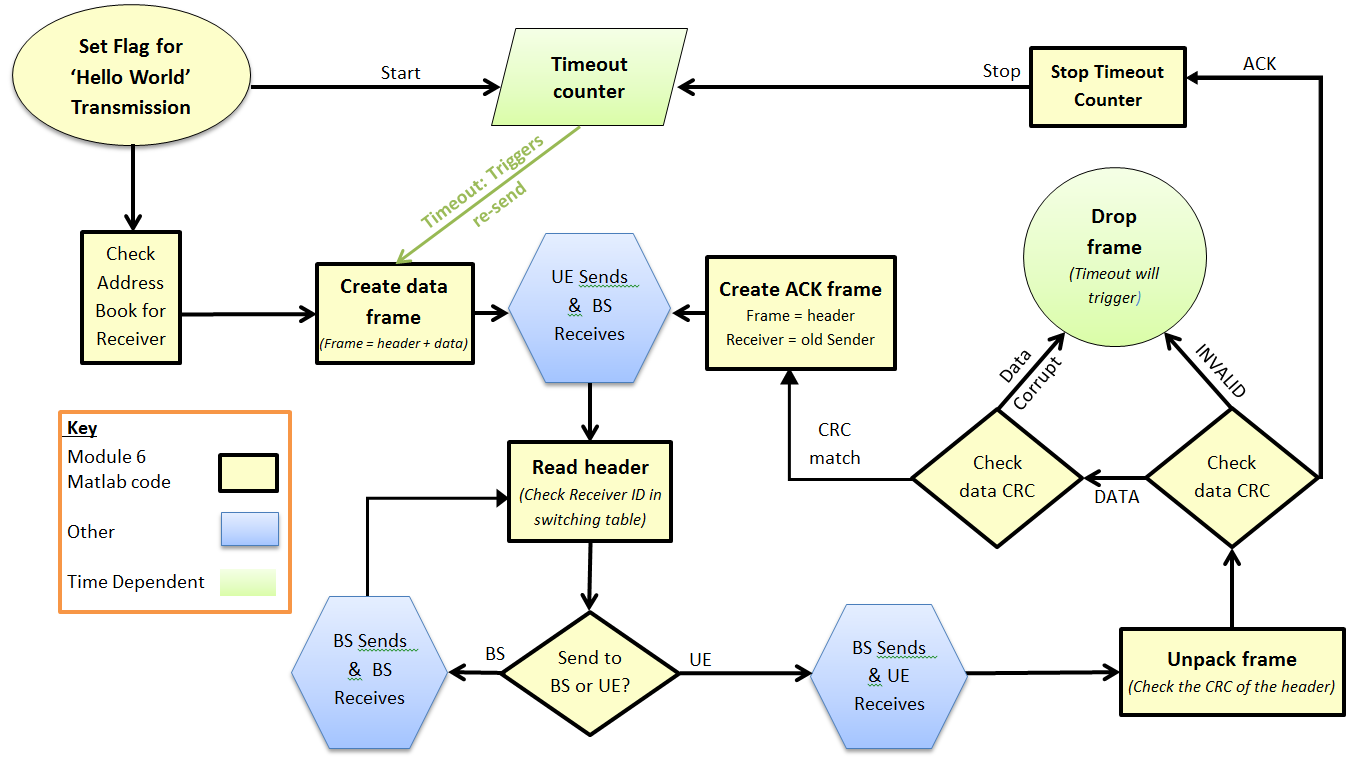
\includegraphics[width=0.8\textwidth]{State_Machine_yellow.PNG}
    \caption{State Machine of the transmission of a package }
    \label{fig:stateMachine}
\end{figure}

\begin{figure}[ht]
    \centering
    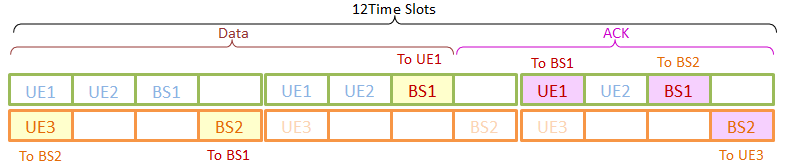
\includegraphics[width=0.8\textwidth]{ACK_timeout_long.PNG}
    \caption{Diagram of an example of the longest time between a UE transmitting frame of data and receiving the corresponding ACK}
    \label{fig:ACKtimelong}
\end{figure}

\begin{figure}[ht]
    \centering
    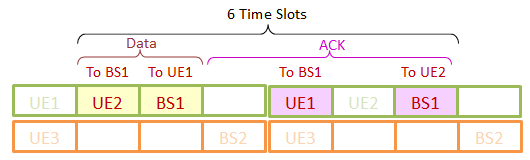
\includegraphics[width=0.8\textwidth]{ACK_timeout_short.PNG}
    \caption{Diagram of the shortest time between a UE transmitting a frame of data and receiving the corresponding ACK}
    \label{fig:ACKtimeshort}
\end{figure}

\begin{figure}[ht]
    \centering
    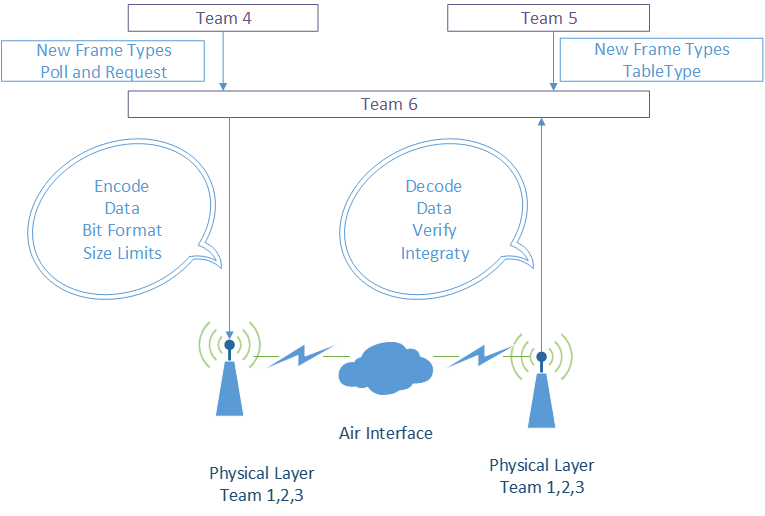
\includegraphics[width=0.8\textwidth]{Interface_diagram.PNG}
    \caption{Diagram of how Module 6 interfaces with the rest of the network}
    \label{fig:Interface}
\end{figure}